\documentclass[10pt]{article}
\usepackage{SIRC}
\usepackage{mathptmx}
\usepackage{subfigure}
\usepackage{float}
\usepackage{graphicx}
\usepackage{harvard}
\usepackage{url}


\begin{document}


%The title of our paper
\title{The View from the Chathams: \\ Geovisualisation of Web Site Hits using Google Earth\textsuperscript{\texttrademark}}

%The author(s) of our paper
\author{Nigel Stanger\textsuperscript{1}}

%Special command for formatting of the Author's name etc. First parameter is the superscript number. Second are the details
\Address{1}{Department of Information Science \\
University of Otago. Dunedin, New Zealand \\
Phone: +64 3 479-8179 Fax: +64 3 479-8311 \\
Email: nstanger@infoscience.otago.ac.nz}

%Include where our paper was presented.
\PresentedAt

\begin{abstract}
A useful approach to visualising the geographical distribution of web site hits is to geolocate the IP addresses of hits and plot them on a world map. In this paper we examine the efficacy of Google Earth for this purpose.
\end{abstract}

%Format our keywords
\Keywords{web traffic, geolocation, geovisualisation, digital repository, Google Earth}


\section{INTRODUCTION}

When administering a web site, it is normal to want information on the nature of traffic to the site. Information on the geographic sources of traffic can be particularly useful in the right context. For example, an e-commerce site might wish to determine the geographical distribution of visitors to the site, so as to decide where best to target marketing resources. One approach to doing so is to plot the distribution on a map. Geographical information systems (GIS) were already being used for these kinds of purposes prior to the advent of the World Wide Web \cite{Beau-JR-1991-GIS}, and it is a natural extension to apply these ideas to online geovisualisation of web site hits.

In November 2005 the author implemented a pilot digital institutional repository\footnote{\url{http://eprints.otago.ac.nz/}} for the University of Otago School of Business \cite{Stan-N-2006-running}, using the GNU EPrints\footnote{\url{http://www.eprints.org/}} repository management software. This repository quickly attracted interest from around the world and the number of abstract views and document downloads began to steadily increase. There was great interest within the University in tracking this increase, particularly with respect to where in the world the hits were coming from. The EPrints statistics management software developed at the University of Tasmania \cite{Sale-A-2006-stats} proved very useful in this regard, providing detailed per-country download statistics, as illustrated in Figure~\ref{fig-tas-stats}. However, while this display provides an ordered ranking of the number of hits from each country, it does not provide any further detail below the country level, nor does it provide any visual clues as to the spatial distribution of hit sources around the globe.


\begin{figure}
	\centering
	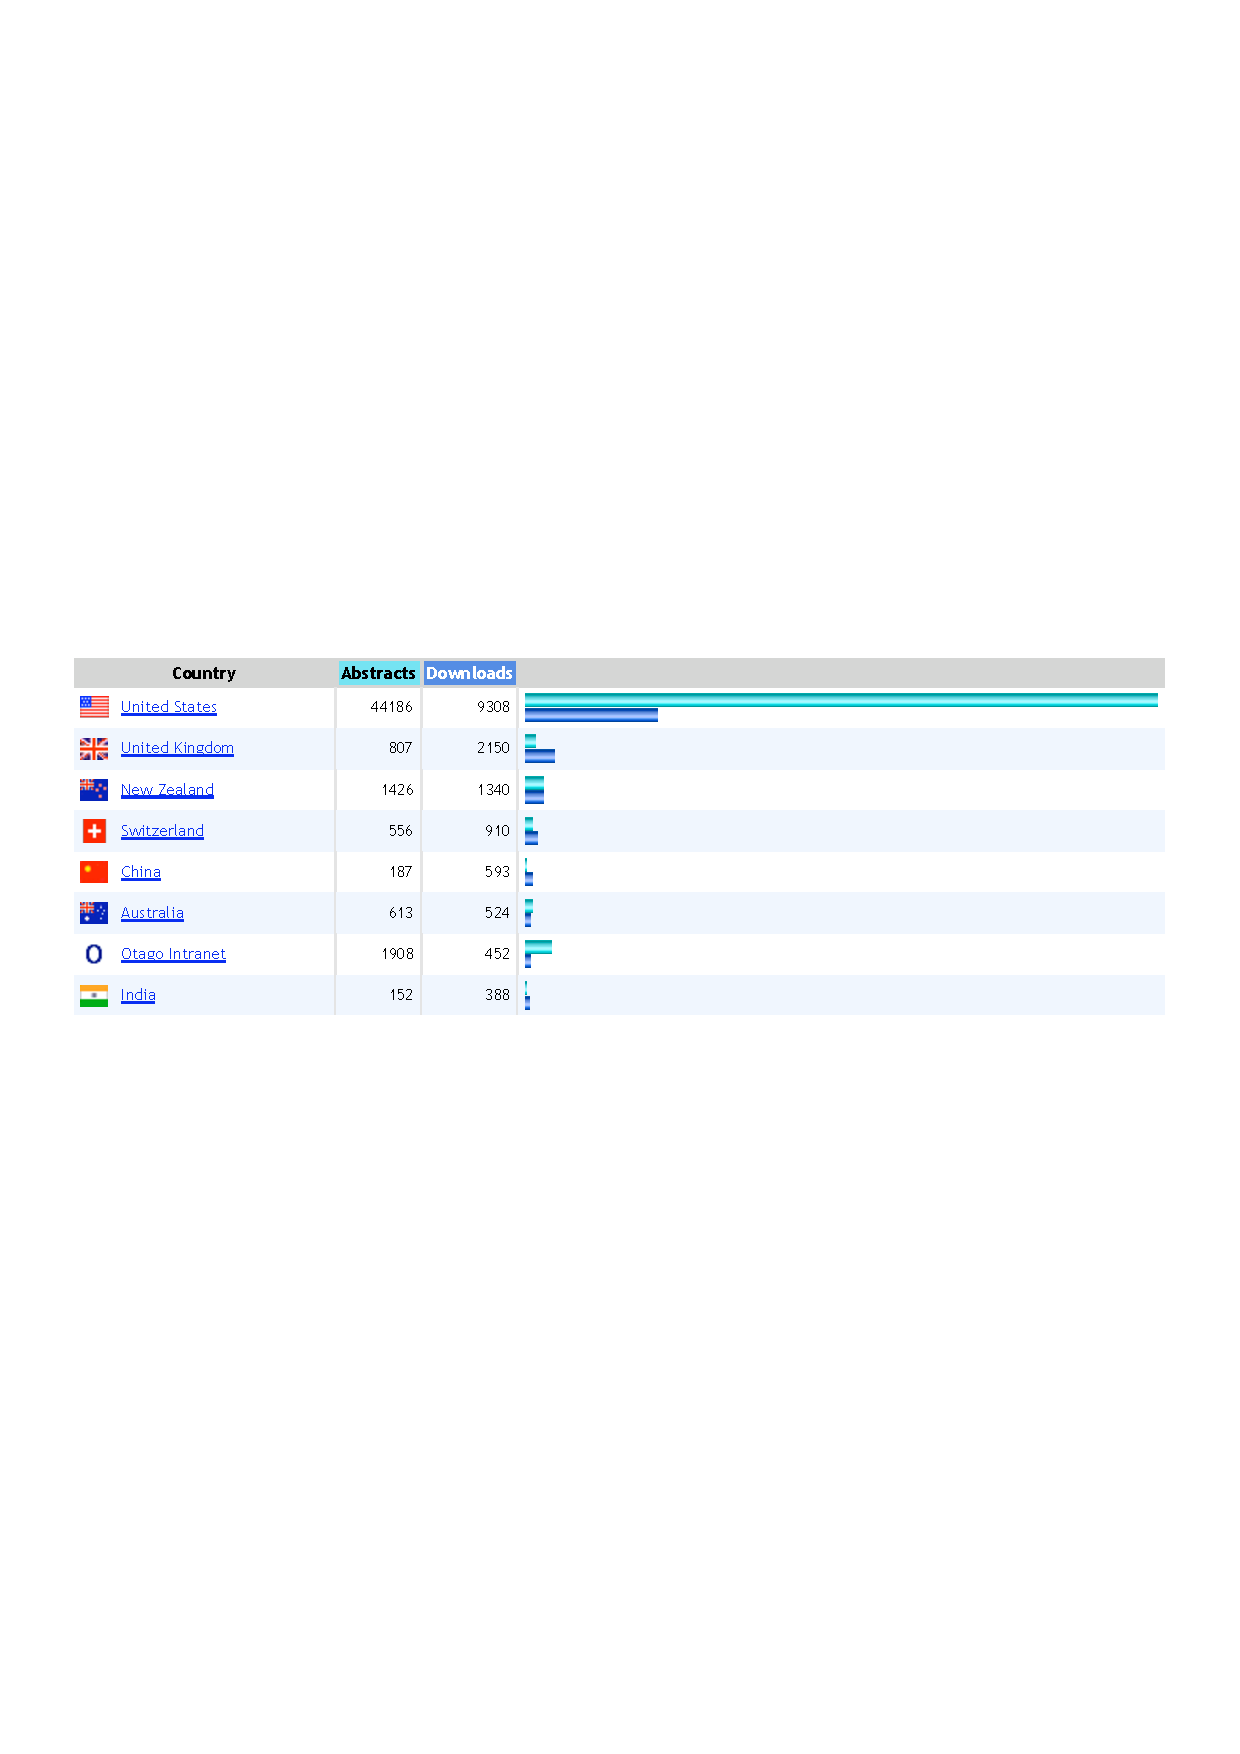
\includegraphics[width=\textwidth,keepaspectratio]{tasmania_stats}
	\caption{\textit{A portion of the by-country traffic display for the Otago EPrints repository, generated by the Tasmania statistics software
	\protect\cite{Sale-A-2006-stats}}}
	\label{fig-tas-stats}
\end{figure}


The author therefore began to explore techniques for plotting the repository's web traffic onto a world map. There have been several prior efforts to geovisualise web activity. \citeasnoun{Lamm-SE-1996-webvis} developed a sophisticated system for real-time visualisation of web traffic on a 3D globe, but this was intended for use within a virtual reality CAVE \cite{CrNe-C-1992-CAVE}, thus limiting its general applicability. \citeasnoun{Papa-N-1998-Palantir} described a similar 2D system called \emph{Palantir}, which was written as a Java applet and was thus able to run within any Java-enabled web browser. \citeasnoun[pp.\ 100--103]{Dodg-M-2001-cybermap} describe these and several other related systems for mapping Web and Internet traffic.

These early systems provided impressive visualisations, but suffered from a distinct limitation in that there was no public infrastructure in place for geolocating IP addresses (that is, translating them into latitude/longitude coordinates). They generally used \texttt{whois} lookups or parsed the domain name in an attempt to guess the country of origin, with fairly crude results \cite{Lamm-SE-1996-webvis}. Locations outside the United States were typically aggregated by country and mapped to the capital city \cite{Lamm-SE-1996-webvis,Papa-N-1998-Palantir,Jian-B-2000-cybermap}. Reasonably accurate and detailed databases were commercially available at the time \cite[p.\ 1466]{Lamm-SE-1996-webvis}, but were not generally available to the public at large, thus limiting their utility.

The situation has improved considerably in the last five years, however, with the advent of freely available and reasonably accurate geolocation services\footnote{Such as \url{http://www.maxmind.com/} or \url{http://www.ip2location.com/}.} with worldwide coverage and city-level resolution. For example, Maxmind's \emph{GeoLite City} database is freely available and claims to provide ``60\% accuracy on a city level for the US within a 25 mile radius'' \cite{Maxm-G-2006-GeoLiteCity}. Their commercial \emph{GeoIP City} database claims 80\% accuracy for the same parameters. This means that it is now feasible to generate reasonably precise displays of the geographic origins of web site hits.

Another exciting development in recent years has been the advent of powerful, freely available map visualisation software from Google, Inc. Google Maps and Google Earth both enable dynamic and sophisticated interaction with detailed maps and satellite imagery of the Earth. Google Maps is 2D and works in any web browser, while Google Earth is 3D and runs as a separate application. Both run on commonly available hardware. The arrival of this software means that almost anyone can create sophisticated map visualisations with relatively little effort. Google Earth is of particular interest because of its powerful 3D visualisation capabilities.

The remainder of the paper explores the efficacy of various approaches to geovisualising web site hits, focusing primarily on Google Earth. Section~\ref{sec-two-dimensional} briefly discusses four representative approaches to 2D geovisualisation of web site hits, and the limitations inherent with these approaches. Section~\ref{google-earth} then discusses the author's experience of building 3D web hit geovisualisations using Google Earth. Issues that were encountered are discussed in Section~\ref{sec-issues}.


\section{TWO-DIMENSIONAL APPROACHES}
\label{sec-two-dimensional}

The author initially focused on 2D map visualisations that could be easily displayed within a web browser, such as that shown in Figure~\ref{fig-image}. Four representative techniques, corresponding to different distribution styles \cite{Wood-J-1996-vis,MacE-AM-1998-GIS}, were identified for implementing these visualisations:
\begin{enumerate}

	\item \emph{server-side image generation}, where points were plotted onto a base map image at the server, and the single combined image returned to the browser;
	
	\item \emph{server-side image overlay}, where one or more transparent overlay images were generated at the server and returned to the browser along with a base map image, then composited at the browser;
	
	\item \emph{server-side HTML overlay}, where one or more overlays comprising absolutely positioned HTML elements (e.g., \texttt{DIV} elements) were generated at the server and returned to the browser along with a base map image, then composited at the browser; and
	
	\item \emph{Google Maps}, where the browser asynchronously requested map images and overlay data from the server, then generated the final map at the browser.

\end{enumerate}
The scalability of these four techniques was tested in a series of experiments\footnote{A paper discussing the results of these experiments is currently under review.}, to see whether they could handle the volumes of web hit data that might be generated by a typical web site.


\begin{figure}
	\centering
	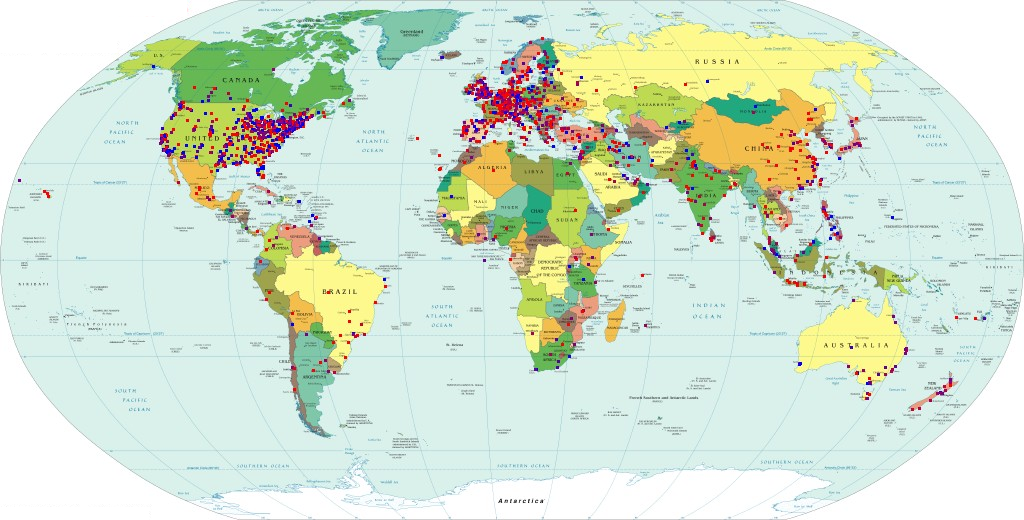
\includegraphics[width=\textwidth,keepaspectratio]{ImageGeneration-full}
	\caption{\textit{A typical 2D map displaying web hits from the Otago EPrints repository}}
	\label{fig-image}
\end{figure}


The server-side image generation and image overlay techniques were found to be the best performers, as shown in Figure~\ref{fig-combined-time}. Maps were relatively easy to generate and the two techniques scaled well to extremely large numbers of data points, taking on the order of twenty seconds to generate a map with about one million (\(2^{20}\)) points. This performance advantage was offset, however, by the maps' static nature and lack of interactivity.


\begin{figure}
	\centering
	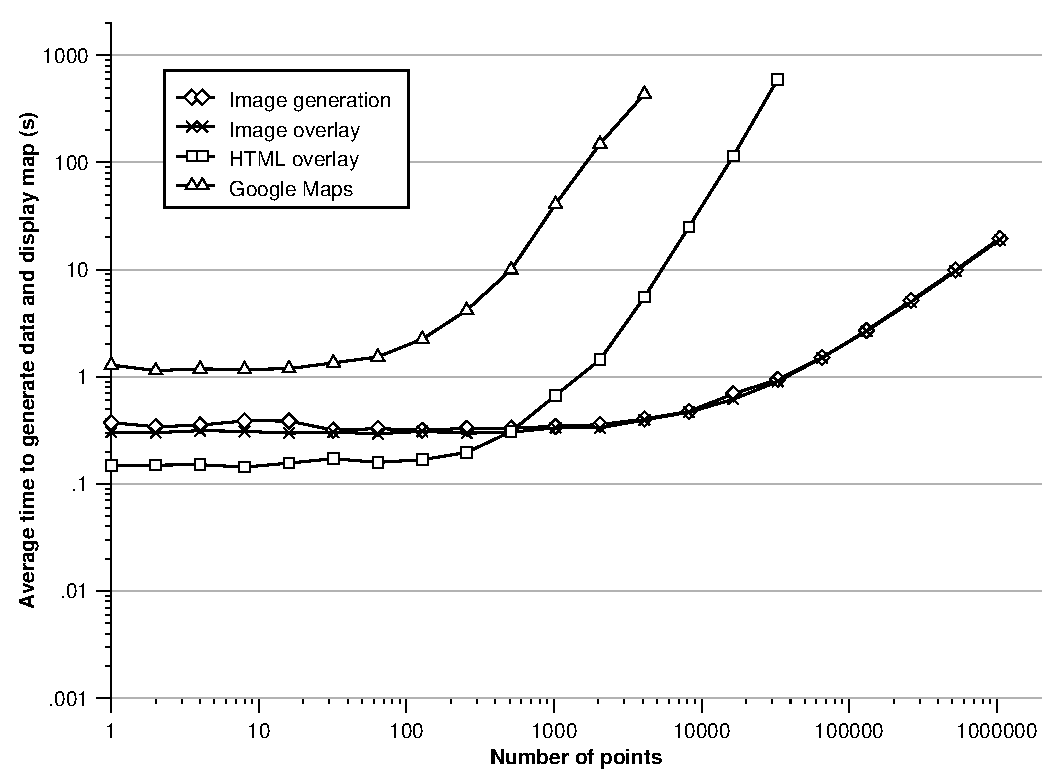
\includegraphics[scale=0.55]{combined_time}
	\caption{\textit{Comparison of page load time for four online map generation techniques (log-log scale)}}
	\label{fig-combined-time}
\end{figure}


It was expected that Google Maps would provide a more dynamic experience, but as can be seen in Figure~\ref{fig-combined-time}, it was the worst performer of the group, taking over seven minutes to load a page with only 4,096 points! This was most likely due to memory overload within the browser's JavaScript engine, due to the amount of data being manipulated. Google Maps was thus eliminated as a serious contender.


\section{GOOGLE EARTH}
\label{google-earth}

Google Earth is a free ``Earth explorer'' that combines satellite imagery, maps and the Google search engine into a powerful tool for geovisualisation. Google Earth runs under Windows, Mac OS X and Linux, on any reasonably modern PC with a 3D video card. Users can easily create and apply their own overlays, thus gaining much of the visualisation power of a GIS without the associated complexity. Google Earth has been used for many different applications, including topographical analysis \cite{USGS-2006-topo}, geology \cite{Thom-K-2006-GSA,dePa-DG-2006-GSA}, palaeogeography and archaeology. It is also an obvious ``mass market'' successor to the earlier resource-intensive 3D geovisualisation systems developed by the likes of \citeasnoun{Lamm-SE-1996-webvis}.

Google Earth overlays are specified using an XML dialect called Keyhole Markup Language (KML), and can be displayed or hidden at will within the Google Earth application. KML files are relatively simple to generate, and there are many available for download from the Internet. In addition to static KML files, web sites can provide \emph{network links}, which are dynamic data sources generated by server-side scripts and accessed remotely by the Google Earth application. This enables automatic refreshing of the data on a regular basis.

The author's first KML effort was a simple port of the 2D visualisation shown in Figure~\ref{fig-image}. Traffic data were extracted from the Otago EPrints repository statistics database (which were in turn derived from the Apache web server logs). The IP addresses were geolocated using MaxMind's free GeoLite City database, and the number of abstract views and document downloads for each distinct geographical location was accumulated. A KML icon was then generated for each distinct location, coloured according to the proportion of abstract views (blue) versus document downloads (red) at that location. This produced an interesting display, but provided no additional benefit beyond ``looking cool''. In particular, it took no advantage of the third dimension that was now on offer.

The next step was to use this third dimension to display the traffic volume information inherent in the data set. For each distinct location, two KML polygons were generated, a blue one representing abstract views and a red one representing document downloads. The polygons were extruded vertically by 1,000 metres per hit, producing a 3D bar. This approach produced visually stunning images such as those shown in Figure~\ref{fig-google-bars}. The display is reminiscent of the 3D web traffic visualisations produced by \citeasnoun{Lamm-SE-1996-webvis}, but is accessible to a much broader audience. The bar visualisation is highly interactive, and also highly informative when combined with the icon visualisation described in the previous paragraph. For example, while it was apparent from the icon view that the Otago repository had been frequently accessed from Europe, there was no clear indication of the relative levels of traffic across Europe. The bar view, on the other hand, instantly revealed very high traffic levels from Southampton, London, Manchester and Stockholm, in particular.


\begin{figure}
	\centering
	\subfigure[\textit{View from Paris across the English Channel; the tall bars over England are (from left to right) Southampton, Wolverhampton, Manchester and London}]{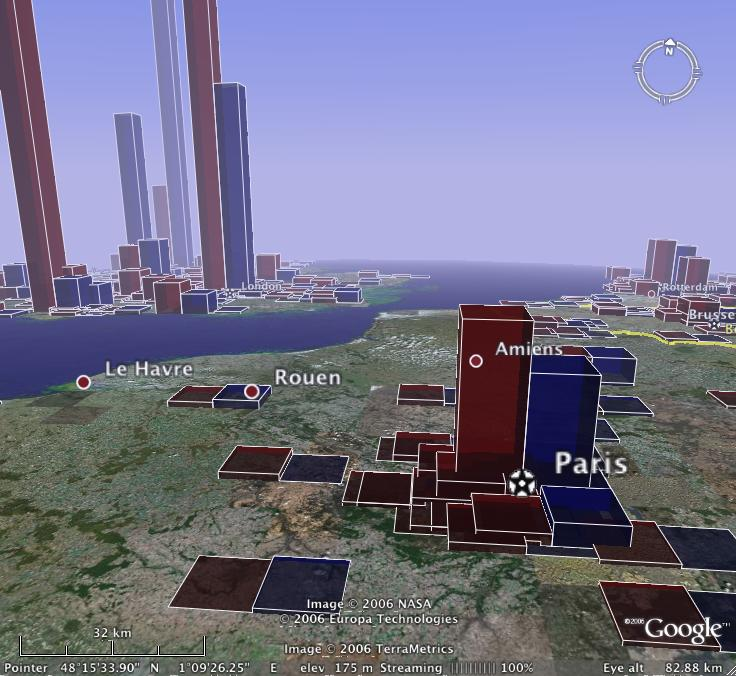
\includegraphics[scale=0.4]{bars_Paris}}
	
	\subfigure[\textit{View of New Zealand from the Chatham Islands; note the large spike of non-geolocated traffic in the Marlborough Sounds}]{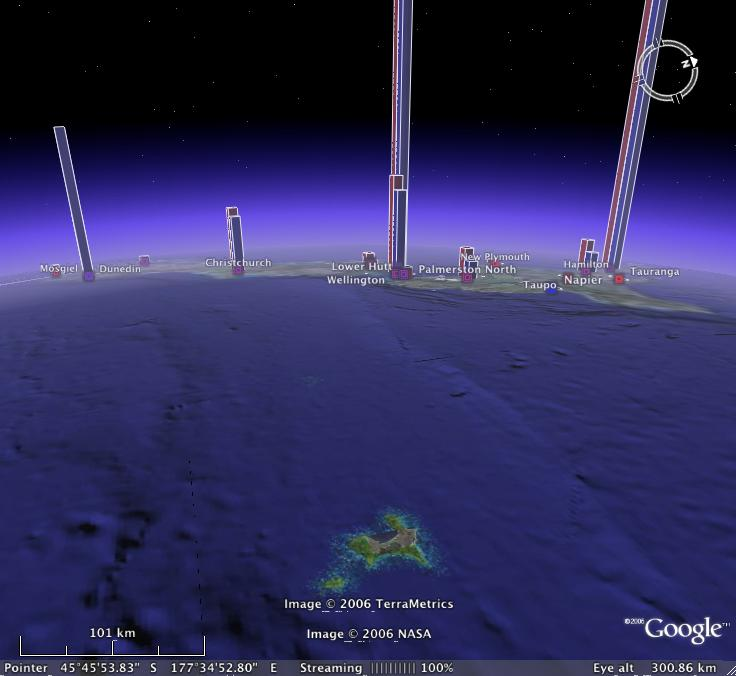
\includegraphics[scale=0.4]{bars_Chathams}}
	\caption{\textit{Google Earth geovisualisations of web traffic to the Otago EPrints digital repository}}
	\label{fig-google-bars}
\end{figure}


\section{ISSUES ENCOUNTERED}
\label{sec-issues}


\subsection{Geolocation}

Several issues arose from the geolocation tools used. The geolocation process is independent of the visualisation method, so these issues will affect any attempt at geovisualising data derived from IP addresses.

First, IP address ranges are continually changing and being reassigned across organisations. This means that the physical location of an IP address may change over time. These changes will eventually be reflected in the various geolocation databases, so the same source data may produce different results at different points in time. However, this is only a significant issue if precise measurements are required. In the case of the Otago EPrints repository, for example, such precision is not as important as the ability to easily identify overall access patterns.

A second issue is that of homonyms and synonyms. \emph{Homonyms} occur when the same name is associated with two or more distinct locations. If the homonyms occur in distinct countries (e.g., London, UK versus London, Canada), then the country name can be used to disambiguate the two. If the homonyms occur within the same country (e.g., Stafford, Georgia versus Stafford, Texas), then more care must be applied. Disambiguation based on the geographic coordinates is an obvious solution, but this is complicated somewhat when the geolocation database returns slightly different coordinates for IP addresses in the same city. \emph{Synonyms} occur when there are multiple names for the same geographic location. Examples noted by the author include Beijing/Peking, Mumbai/Bombay, and somewhat disconcertingly, Louisville/LOUISVILLE. The latter case could be remedied by case normalisation, but there is no simple solution to the other cases.

Third, many IP addresses cannot be successfully geolocated below the country level. In these cases, the geolocation database appears to returns a default location in the approximate geographical centre of the country in question. As a consequence, very large apparent traffic rates pop up in some extremely odd places, such as a wheat field in Kansas, the middle of the Sahara Desert or the Marlborough Sounds, or a yurt Outer Mongolia. There appears to be no satisfactory solution to this issue other than simply omitting these data, or perhaps placing them into a separate KML ``folder'', which can then be displayed separately.

A final issue arises from the way that traffic data for the Otago EPrints repository were gathered. Two custom ``countries'' were created representing traffic from the Otago intranet and repository administrative staff, respectively. The former was done in order to track interest from within the University, while the latter was done to prevent routine administrative access from artificially inflating the Otago intranet figures. Since these are stored as distinct ``countries'' in the statistics database, visualisation generators must special-case them to avoid plotting them as distinct entries at the same geographic location. In this particular case, the two extra ``countries'' were re-mapped to Dunedin.


\subsection{Google Earth}

Only one significant issue relating to Google Earth itself has been noted so far: KML supports only latitude/longitude coordinates. This is not an issue when simply plotting an icon at a given location, but it does cause a problem when drawing a polygon whose vertices are offset a constant distance relative to that location. For example, in the original version of the bar visualisation, the north and south edges of each bar were offset \(\pm\)0.075 degrees, or approximately 8\,km, from the actual location. A similar offset scheme was used for the east and west edges of the bar. However, the size of a degree of longitude shrinks as one moves from the equator towards the poles, so the bars were square at the equator (approximately 16\,km on a side), but became progressively more oblong at higher latitudes.

Fortunately it is relatively simple to compensate for this effect. Using simple trigonometry, a lookup table can be derived that provides a latitude adjustment factor at whatever level of resolution is desired (e.g., one degree intervals). This can then be used as a longitude multiplier when calculating polygon coordinates relative to the base location.


\section{CONCLUSIONS}

Google Earth has proven to be an effective tool for geovisualising web traffic, generating visualisations that are highly interactive and visually spectacular. While it has been applied to only a single web site (the Otago EPrints digital repository), the results should be readily generalisable to any web site that keeps adequate traffic logs, as all web sites use essentially the same underlying mechanisms.

Certainly the author has only scratched the surface of what may be possible with this tool. The current visualisations are generated as static KML files, which could raise scalability issues for very large data sets. One solution might be to implement the visualisations as network links that return only data that are visible from the current viewpoint. The current visualisations also display all the available data; it would be useful to limit this to traffic for specific eprints, countries or time periods. Finally, version 2.1 of KML adds support for temporal animation of overlays. This adds a fourth dimension to the three already available and thus opens the door to even more compelling visualisations.


\section*{ACKNOWLEDGEMENTS}

``Google'', ``Google Maps'' and ``Google Earth'' are all trademarks of Google, Inc. Neither the author nor this research are affiliated with Google, Inc.\ in any way. The map shown in Figure~\ref{fig-image} has been placed into the public domain by the \citeasnoun{CIA-WFB-2006}.


\bibliographystyle{dcu}
\bibliography{SIRC}

\end{document}
